\chapter{References}
\printbibliography[heading=none]

\chapter{Appendix}
\section{Submission File Structure}
\todo{Write section}

\section{Running the Code}
\label{sec:running-the-code}
Install rustup and rustc 1.25.0-nightly (0c6091fbd 2018-02-04) compiler: \\
\texttt{curl https://sh.rustup.rs -sSf | sh -s -- -y --default-toolchain nightly-2018-03-05} \\

Verify the version is correct using: \\
\texttt{rustc --version} \\

Create a new crate and write sequential code: \\
\texttt{cargo init} \\

Under \texttt{[dependencies]} in \texttt{Cargo.toml}, add: \\
\texttt{auto\_parallelise=\{version="*", git="https://github.com/MichaelOultram/Auto\_Parallelise/"\}} \\

At the top of your \texttt{lib.rs} or \texttt{main.rs} file, add: \\
\texttt{\#![feature(plugin)]} \\
\texttt{\#![plugin(auto\_parallelise)]} \\

At the top of every function, add: \\
\texttt{\#[autoparallelise]} \\

Compile the code once to run the analysis stage: \\
\texttt{cargo build --release} \\

Normally you would compile the code again with the same command to apply the modifications but due to a bug in the rust nightly compiler (\href{https://github.com/rust-lang/rust/issues/46489}{$\#46489$}), this doesn't work. Instead you must pipe stdout into a file: \\
\texttt{cargo build --release > parallel\_code.rs} \\

Normally you would just run the parallelised code but due to the bug, you will need to create a new project and copy \texttt{parallel\_code.rs} along with any imports. Then you can: \\
\texttt{cargo run --release}

%\section{Project Proposal and Scientific Paper}
%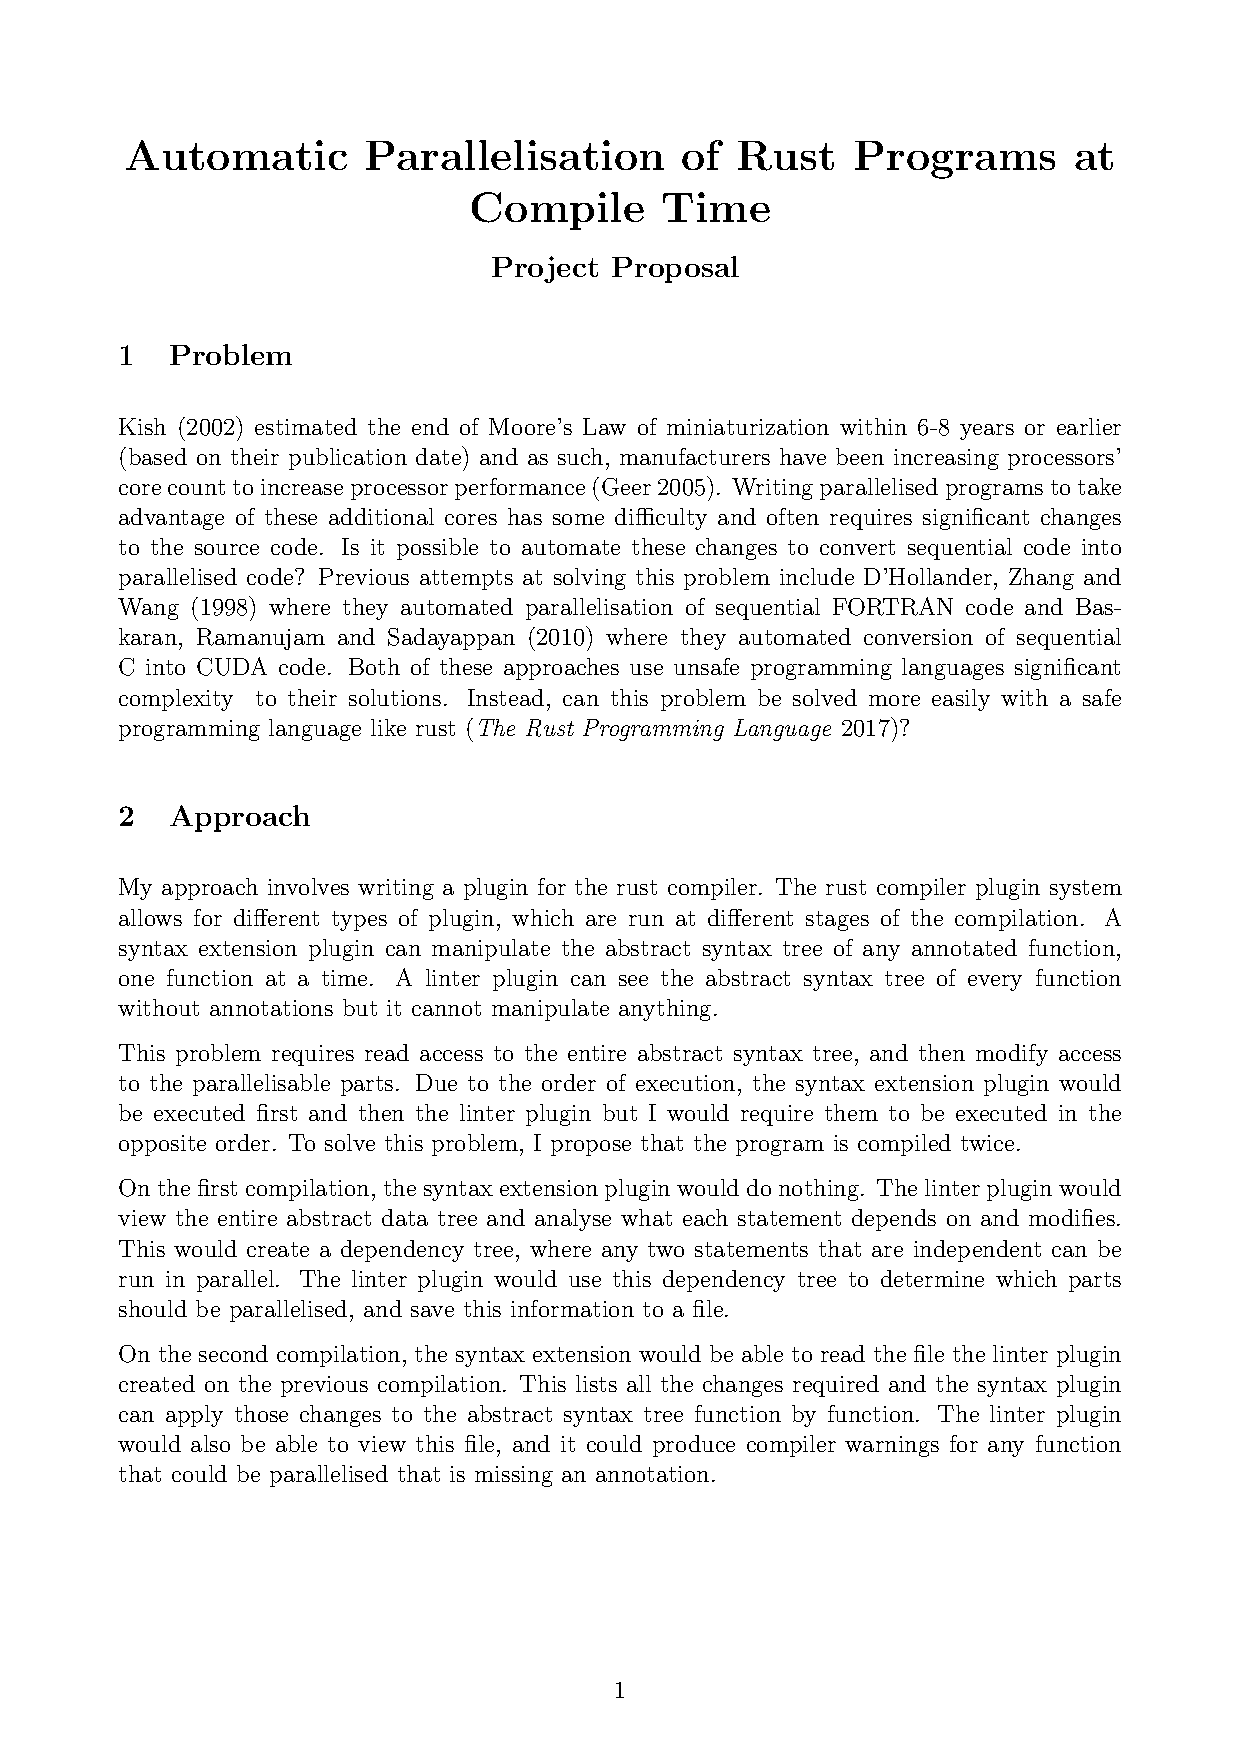
\includepdf[pages=-]{../0-Proposal/main.pdf}
%
\includepdf[pages=-]{../1-Scientific-Paper//main.pdf}

\section{Rust Compiler Types}
\begin{code}
    % FnKind Enum
    \inputcode{rust/src/libsyntax/visit.rs}{34}{43}
    \caption{\texttt{FnKind} enum}
    \label{lst:rustc-FnKind}
\end{code}

\begin{code}
    % Block Struct
    \inputcode{rust/src/libsyntax/ast.rs}{489}{497}
    \caption{\texttt{Block} struct}
    \label{lst:rustc-Block}
\end{code}

\begin{code}
    % Stmt Struct
    \inputcode{rust/src/libsyntax/ast.rs}{781}{785}
    \caption{\texttt{Stmt} struct}
    \label{lst:rustc-Stmt}
\end{code}

\begin{code}
    % StmtKind enum
    \inputcode{rust/src/libsyntax/ast.rs}{815}{828}
    \caption{\texttt{StmtKind} enum}
    \label{lst:rustc-StmtKind}
\end{code}

\begin{code}
    % Expr Struct
    \inputcode{rust/src/libsyntax/ast.rs}{899}{904}
    \caption{\texttt{Expr} struct}
    \label{lst:rustc-Expr}
\end{code}

\begin{code}
    % ExprKind enum
    \inputcode{rust/src/libsyntax/ast.rs}{987}{1122}
    \caption{\texttt{ExprKind} enum}
    \label{lst:rustc-ExprKind}
\end{code}

\begin{code}
    % SpanData Struct
    \inputcode{rust/src/libsyntax_pos/lib.rs}{143}{149}
    \caption{\texttt{SpanData} struct}
    \label{lst:rustc-SpanData}
\end{code}
